\documentclass[a4paper]{article}

\usepackage{mathtools} % математические формулы
\usepackage[T1,T2A]{fontenc} % кириллица
\usepackage[utf8]{inputenc} % кодировка шрифта кириллицы
\usepackage{indentfirst} %делать отступ в начале параграфа
\usepackage{enumerate} % нумерация списков
\usepackage{tabularx} % таблицы
\usepackage[english,russian]{babel} % вставка стороннего текста
\usepackage[12pt]{extsizes}
\usepackage{amsthm, amssymb, amsmath, amsfonts, nccmath, empheq}
\usepackage{color,colortbl} 
\usepackage[warn]{mathtext}
\usepackage{tocloft}  % для отточий в оглавлении
\linespread{1.5}
\usepackage{setspace} % для пробелов между линий
\usepackage{cmap}


\onehalfspacing
\usepackage{float}
\usepackage{graphicx}
\graphicspath{{pictures/}}
\DeclareGraphicsExtensions{.pdf,.png,.jpg}
\usepackage[left=25mm,right=25mm,
    top=2cm,bottom=30mm,bindingoffset=0cm]{geometry}
\renewcommand{\cftsecleader}{\cftdotfill{\cftdotsep}}

\usepackage{hyperref} % для гиперссылки на гитхаб

\author{Тырыкин Я. А. }
\date{March 2021}

\begin{document}
\begin{titlepage}
    \begin{center}
        \mbox{\normalsize{Санкт-Петербургский Политехнический Университет имени Петра Великого}}\\
        \normalsize{Институт Прикладной Математики и Механики}\\
        \large{\textbf{Кафедра "Прикладная Математика"}}
        
        \vfill
        
        \textbf{\Large{Отчет по лабораторным работам №6}}\\
        \textbf{\large{по дисциплине}}\\
        \textbf{\large"Математическая Статистика"}
        
        \vfill
        \raggedleft{Выполнил студент:}\\
        \raggedleft{Тырыкин Я. А.}\\
        \raggedleft{группа 5030102/80401}\\
        \raggedleft{Проверил:}\\
        \raggedleft{к.ф.-м.н., доцент}\\
        \raggedleft{Баженов А. Н.}\\
        
        \vfill
    
    \end{center}
    
    \begin{center} 
        Санкт-Петербург \\
        2021 
    \end{center}
\end{titlepage}
\newpage

% страница со списком графиков
\begin{center}
    \listoffigures
\end{center}
\newpage

\section{Постановка задачи}
    Найти оценки коэффициентов линейной регрессии $y_i = a + bx_i + e_i$, используя 20 точек на отрезке $[-1.8, 2]$ с равномерным шагом равным 0.2. Ошибку $e_i$ считается нормально распределённой с параметрами (0, 1). В качестве эталонной зависимости берется $y_i = 2 + 2x_i + e_i$. При построении оценок  коэффициентов используются два критерия: критерий наименьших квадратов и критерий наименьших модулей. То же самое проделывается для выборки, у которой в значения $y_1$ и $y_{20}$ вносятся возмущения 10 и -10.

\section{Теория}

    \subsection{Простая линейная регрессия}
    
        \subsubsection{Модель простой линейной регрессии}
    
        Регрессионную модель описания данных называют \textit{простой линейной регрессией}, если 
        
        \begin{equation} \label{simpl_regr}
            y_i = \beta_0 + \beta_1x_i + e_i, i = 1, ..., n
        \end{equation}
        
        где $x_i, ..., x_n$ - заданные числа (значения фактора); $y_i, ..., y_n$ - наблюдаемые значения отклика; $\epsilon_0, ..., \epsilon_n$ - независимые, нормально распределенные $N(0, \sigma)$ с нулевым математическим ожиданием и одинаковой (неизвестной) дисперсией случайные величины (ненаблюдаемые); $\beta_0, ..., \beta_n$ - неизвестные параметры, подлежащие оцениванию.
        
        В модели (\ref{simpl_regr}) отклик $y$ зависит зависит от одного фактора $x$, и весь разброс экспериментальных точек объясняется только погрешностями наблюдений (результатов измерений) отклика $x$. Погрешности результатов измерения $x$ в этой модели полагают существенно меньшими погрешностей результатов измерений $y$, так что ими можно пренебречь.

        \subsubsection{Метод наименьших квадратов}
        
       При оценивании параметров регрессионной модели используют различные методы. Один из наиболее распрстранённых подходов заключается в следующем: вводится мера (критерий) рассогласования отклика  регрессионной функции, и оценки параметров регрессии определяются так, чтобы сделать это рассогласование наименьшим. Достаточно простые расчётные формулы для оценок получают при выборе критерия в виде суммы квадратов отклонений значений отклика от значений регрессионной функции (сумма квадратов остатков):
        
        \begin{equation} \label{mnk}
            Q(\beta_0, \beta_1) = \sum\limits_{i=1}^n{\epsilon^{2}_{i}} = \sum\limits_{i=1}^n{(y_i - \beta_0 - \beta_1 x_1)^{2}} \rightarrow \min_{\beta_0, \beta_1}
        \end{equation}
        
        Задача минимизации квадратичного критерия (\ref{mnk}) носит название задачи \textit{метода наименьших квадратов} (МНК), а оценки $\widehat{\beta_0}$, $\widehat{\beta_1}$ параметров $\beta_0$ и $\beta_1$, реализующие минимум критерия (\ref{mnk}) называют \textit{МНК-оценками}. Данный метод, вообще говоря, может применяться для аппроксимации заданного набора экспериментальных данных линейной комбинацией линейно независимых функций, размер которой не превосходит мощности множества данных (в случае равенства получаем интерполяцию).\\
        
        \textit{Оптимальность}
        
        Критерием оптимальности подобранной аппроксимации является 2 $l^{2}$-норма, точнее, для простоты вычисления, её квадрат:
        
        \begin{equation} \label{square norm mnk}
            \sum\limits_{i=1}^{n}{{||\lambda_i f_i(\{x_n\}) - \{y_n\}||}_{l^2}^{2}} \rightarrow_{\lambda_i} min
        \end{equation}
        
        Минимум ищется по коэффициентам линейной комбинации, исходя из критерия равенства нулю градиента и положительной определённости Якобиана.

        
        \subsubsection{Расчетный формулы для МНК-оценок}
        
        МНК-оценки параметров $\beta_0$ и $\beta_1$ находятся из условия обращения функции $Q(\beta_0, \beta_1)$ в минимум.
        
        Для нахождения МНК-оценок $\widehat{\beta_0}$ и $\widehat{\beta_1}$ выпишем необходимые условия экстремума: \\
        
        \begin{equation} \label{extremum cond}
            \begin{cases}
                \frac{\delta Q}{\delta \beta_0} = -2 \sum\limits_{i=1}^{n}{y_i - \beta_0 - \beta_1 x_i} = 0 \\
                \frac{\delta Q}{\delta \beta_1} = -2 \sum\limits_{i=1}^{n}{(y_i - \beta_0 - \beta_1 x_i)} x_i = 0
            \end{cases}
        \end{equation}
        
        Далее для упрощения записи сумм будем опускать индекс суммирования. Из системы \ref{extremum cond} получим: \\
        
        \begin{equation} \label{extremum cond consequence}
            \begin{cases}
                n \widehat{\beta_0} + \widehat{\beta_1}\sum{x_i} = \sum{y_i} \\
                \widehat{\beta_0}\sum{x_i} + \widehat{\beta_1}\sum{(x_i)^2} = \sum{x_i y_i}
            \end{cases}
        \end{equation}
        
        Разделим оба уравнения на $n$: \\
        
        \begin{equation} \label{consequence div n}
            \begin{cases}
                \widehat{\beta_0} + \widehat{\beta_1} (\frac{1}{n} \sum{x_i}) = \frac{1}{n} \sum{y_i} \\
                \widehat{\beta_0}(\frac{1}{n} \sum{x_i}) + \widehat{\beta_1}(\frac{1}{n} \sum{(x_i)^2}) = \frac{1}{n} \sum{x_i y_i}
            \end{cases}
        \end{equation}
        
        и, используя известные статистические обозначения для выборочных первых и вторых начальных моментов: \\
        
        
        \begin{equation} \label{substitutions}
            \overline{x} = \frac{1}{n} \sum{x_i} \text{ }, \text{ } \overline{y} = \frac{1}{n} \sum{y_i} \text{ }, \text{ } \overline{x^2} = \frac{1}{n} \sum{x_i^2} \text{ }, \text{ } \overline{x y} = \frac{1}{n} \sum{x_i y_i} 
        \end{equation}
        
        По итогу получим: \\
        
        \begin{equation} \label{estimations system}
            \begin{cases}
                \widehat{\beta_0} + \widehat{\beta_1} \overline{x} = \overline{y} \\
                \widehat{\beta_0}\overline{x} + \widehat{\beta_1}\overline{x^2} = \overline{x y}
            \end{cases}
        \end{equation}
        
        откуда МНК-оценку $\widehat{\beta_1}$ наклона прямой регрессии находим по формуле Крамера: \\
        
        \begin{equation} \label{beta 1 majorities}
            \widehat{\beta_1} = \frac{\overline{xy} - \overline{x} * \overline{y}}{\overline{x^2} - \overline{y^2}}
        \end{equation}
        
        а МНК-оценку $\widehat{\beta_0}$ определяем непосредственно из первого уравнения системы \ref{estimations system}: \\
        
        \begin{equation} \label{beta 0 majorities}
            \widehat{\beta_0} = \overline{y} - \overline{x} * \widehat{\beta_1}
        \end{equation}
        
    \subsection{Робастные оценки коэффициентов линейной регрессии}
    
    Робастность оценок коэффициентов линейной регрессии (т.е. их устойчивость по отношению к наличию в данных редких, но больших по величине выбросов) может быть обеспечена различными способами. Одним из них является использование метода наименьших модулей вместо метода наименьших квадратов: \\
    
    \textit{Метод наименьших модулей}: \\
    
    \begin{equation} \label{mnk estim 1}
        \sum\limits_{i=1}^{n}{|y_i - \beta_0 - \beta_1 x_1|} \rightarrow \min_{\beta_0, \beta_1}
    \end{equation}
    
    Напомним, что использование метода наименьших модулей в задаче оценивания параметра сдвига распределений приводит к оценке в виде выборочной медианы, обладающей робастными свойствами. В отличие от этого случая и от задач метода наименьших квадратов, на практике задача \ref{mnk estim 1} решается численно. Соответствующие процедуры представлены в некоторых современных пакетах программ по статистическому анализу. \\
    
    Здесь мы рассмотрим простейшую в вычистлительном отношении робастную альтернативу оценкам коэффициентов линейной регрессии по МНК. Для этого сначала запишем выражения для оценок \ref{beta 0 majorities} и \ref{beta 1 majorities} в другом виде: \\
    
    \begin{equation} \label{estimations system robast}
        \begin{cases}
            \widehat{\beta_1} = \frac{\overline{x y} - \overline{x} * \overline{y}}{\overline{x^2} - \overline{y^2}} = \frac{k_{x y}}{s_x^2} = \frac{k_{x y}}{s_x s_y} * \frac{s_y}{s_x} = r_{x y} * \frac{s_y}{s_x}\\
            \widehat{\beta_0} = \overline{y} - \overline{x} \widehat{\beta_1} 
        \end{cases}
    \end{equation}
    
    В формулах \ref{estimations system robast} заменим выборочные средние $\overline{x}$ и $\overline{y}$ соответственно на робастные выборочные медианы $med x$ и $med y$, среднеквадратические отклонения $s_x$ и $s_y$ на робастные нормированные интерквартильные широты $q_x^{*}$ и $q_y^{*}$, выборочный коэффициент корреляции $r_{x y}$ - на знаковый коэффициент корреляции $r_Q$:
    
    \begin{equation} \label{beta 1 R}
        \widehat{\beta_{1R}} = r_Q * \frac{q^*_y}{q^*_x}
    \end{equation}
    
    \begin{equation} \label{beta 0 R}
        \widehat{\beta_{0 R}} = \text{med y} - (\text{med x}) * \widehat{\beta_{1 R}}
    \end{equation}
    
    \begin{equation} \label{r_Q}
        r_Q = \frac{1}{n}\sum\limits^{n}_{i=1}{sgn(x_i - \text{med x})sgn(y_i - \text{med y})}
    \end{equation}
    
    \begin{equation} \label{q_x and q_y}
        q_y^* = \frac{y_{(j)} - y_{(l)}}{k_q(n)} \text{ }, \text{ } q_x^* = \frac{x_{(j)} - x_{(l)}}{k_q(n)} 
    \end{equation}
    
    \begin{equation} \label{l system}
        l = 
        \begin{cases}
            [\frac{n}{4}] + 1 \text{ при } \frac{n}{4} \text{ дробном} \\
            [\frac{n}{4}] \text{ при } \frac{n}{4} \text{ целом}
        \end{cases}
        , \text{ } j = n - l + 1
    \end{equation}
    
     \begin{equation} \label{sgnz}
        \text{sgn z} = 
        \begin{cases}
            1 \text{ при } z > 0 \\
            0 \text{ при } z = 0\\
            -1 \text{ при } z < 0
        \end{cases}
        , \text{ } j = n - l + 1
    \end{equation}
    
    Уравнение регрессии здесь имеет вид: \\
    
    \begin{equation} \label{regression equation}
        y = \widehat{\beta_{0 R}} + \widehat{\beta_{1 R}} x
    \end{equation}
    
    Статистики выборочной медианы и интерквартильной широты обладают робастными свойствами в силу того, что основаны на центральных порядковых статистиках, малочувствительных к большим по величине выбросам в данных. Статистика выборочного знакового коэффициента корреляции робастна, так как знаковая функция $sgn z$ чувствительна не к величине аргумента, а только к его знаку. Отсюда оценка прямой регрессии \ref{regression equation} обладает очевидными робастными свойствами устойчивости к выбросам по координате но она довольно груба. \\
    
    \textit{Оптимальность} \\
    Данный метод основан на минимизации $l^1$ - нормы разности последовательностей полученных кспериментальных данных и значений аппроксимирующей функции.

    
    \subsection{Количественная мера оценки качества регрессии}
    
    Как уже было сказано метод наименьших квадратов (МНК) минимизирует норму в $l^{2}$, а метод наименьших модулей (МНМ) норму в $l^{1}$.\\
    
    Допустим, что мы будем сравнивать между собой полученные оценки для коэффициентов $\beta_0$, $\beta_1$ как модули разностей полученных значений. Тогда в случае, если для какой-то выборки окажется, что по данному критерию оба метода покажут схожие результаты, то может оказаться, что невязка по $l^{2}$-критерию все равно окажется значительно меньше для результатов, полученных с помощью МНК.\\
    
    Это как раз и является следствием того, что рассмотренные методы минимизирует различные нормы. Обратная ситуация, но уже для $l^1$-метрики также может иметь место в некоторых случаях.\\
    
    Соответственно, можно сказать, что $l$-метрики (в данном случае речь о близости прямых) не позволяют делать однозначных выводов о качестве линейной регрессии в смысле близости искомых коэффициентов аппроксимирующих функций.\\
    
\section{Модульная структура программы}

Лабораторная работа выполнена с применением средств языка Python версии 3.7в среде разработки PyCharm IDE (в частности, с применением встроенных методовбиблиотеки SciPy и MatPlotLib). Исходной код лабораторной работы находится поссылке в приложении к отчёту.

\section{Результаты}

    \subsection{Оценки коэффициентов линейной регрессии}
    
        \subsubsection{Выборка без возмущений}
        
        \begin{itemize}
            \item Критерий наименьших квадратов:
            \begin{equation} \label{mnk without noises}
                \widehat{a} \approx 1.73 \text{ }, \text{ } \widehat{b} \approx 1.74
            \end{equation}
            
            \item Критерий наименьших модулей:
            \begin{equation} \label{mnm without noises}
                \widehat{a} \approx 2.31 \text{ }, \text{ } \widehat{b} \approx 2.27
            \end{equation}
            
        \end{itemize}
        
        \begin{figure}[H]
            \centering
            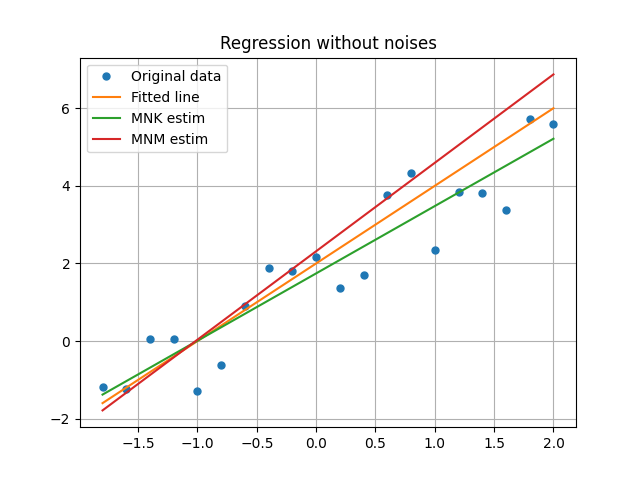
\includegraphics[scale = 0.6]{lab6_without_noise.png}
            \caption{Выборка без возмущений}
            \label{fig:uniform}
        \end{figure}
        
        \subsubsection{Выборка с возмущениями}
        
        \begin{itemize}
            \item Критерий наименьших квадратов:
            \begin{equation} \label{mnk with noises}
                \widehat{a} \approx 2.04 \text{ }, \text{ } \widehat{b} \approx 0.73
            \end{equation}
            
            \item Критерий наименьших модулей:
            \begin{equation} \label{mnm with noises}
                \widehat{a} \approx 2.31 \text{ }, \text{ } \widehat{b} \approx 2.21
            \end{equation}
            
        \end{itemize}
        
        \begin{figure}[H]
            \centering
            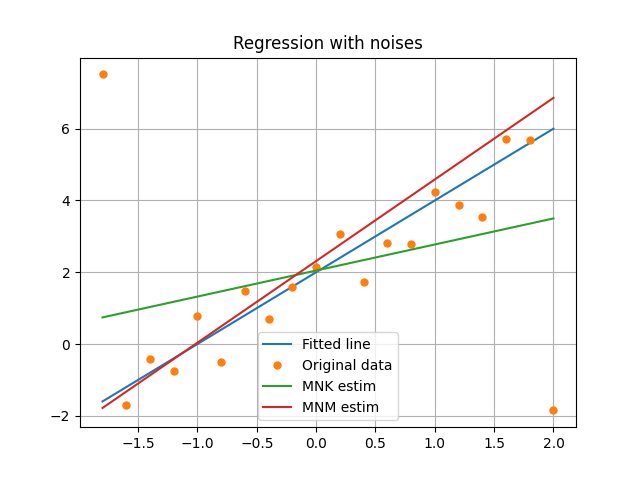
\includegraphics[scale = 0.6]{lab6_with_noises.png}
            \caption{Выборка с возмущениями}
            \label{fig:uniform}
        \end{figure}
        
\section{Обсуждение}
    
    \subsection{Оценки коэффициентов линейной регрессии}
    
        По полученным результатам (и,  в частности, по их графической иллюстрации) можно сказать, что в целом оба критерия (МНК и МНМ) с примерно равноценной точностью оценивают коэффициенты линейной регрессии при отсутствии погрешностей в множестве отклыиков исследуемой системы. Однако при возникновении последних (особенно при сильной зашумленности данных), критерий МНК начинает работать значительно менее точно, что отчетливо видно по значению $\widehat{b}$ и углу наклона соответствующей кривойю Это говорит о его высокой чувствительности к помехам. Критерий МНМ же в условиях второго эксперимента не теряет своей работоспособности.
    
\section{Ресурсы}

    Код программы находится на сайте Github по следующей ссылке: \\
    
    \href{https://github.com/YaroslavAggressive/Mathematical-statistics-lab-works/tree/main}{Ветка с исходным кодом и кодом отчета}

\end{document}
